\documentclass{article}

\usepackage{amsmath}
\usepackage{bm}
\usepackage{etoolbox}
\usepackage{hyperref}
\usepackage{listings}
\usepackage{multicol}
\usepackage{multido}
\usepackage{relsize}
\usepackage{tikz}
\usetikzlibrary{hobby}

\usepackage[utf8]{inputenc}
\usepackage[english]{babel}

\setlength{\parindent}{4em}
\setlength{\parskip}{1em}

\let\oldhat\hat
\renewcommand{\vec}[1]{\pmb{#1}}
\renewcommand{\hat}[1]{\oldhat{\pmb{#1}}}
\newcommand{\undersetvecexp}[4]{
  \underset{ \mathsmaller{#2 \times #3} }
           { \hphantom{{}^{#4}} \vec{#1} ^ {#4} }
}
\newcommand{\kunderset}[3]{
  \underset{ \mathsmaller{#2 \times #3} }
           { #1 }
}
\newcommand{\undersetvec}[3]{ \undersetvecexp{#1}{#2}{#3}{} }
\newcommand{\abs}[1]{\lvert #1 \rvert}
\newcommand{\lnorm}[2]{ {\left\lVert #2 \right\rVert}_#1 }
\newcommand{\lnormexp}[3]{ {\left\lVert #3 \right\rVert}_#1^#2 }
\newcommand{\bigbraces}[1]{ \left\{ #1 \right\} }
\newcommand{\bigbrackets}[1]{ \left[ #1 \right] }
\newcommand{\bigparens}[1]{ \left( #1 \right) }
\newcommand{\kpartial}[2]{ \frac{\partial \, #1}{\partial \, #2} }

\newcommand{\gausswithpeak}[4]{
  ( (#4) *
    (exp( ( -(#1-#2)^2 ) /
          ( 2*(#3^2)   )  ) ) )
}

\newcommand{\KLogisticPdf}[3]{
  % KLogisticPdf{mu}{sdev}{peak}
  (#3) * 4
  * exp( -(x-(#1)) /
          ((#2)*sqrt(3)/pi))
  / ((1 + exp(-(x-(#1)) /
               ((#2)*sqrt(3)/pi)) )**2)
}

\newcommand{\KLogisticCdf}[3]{
  % KLogisticCdf{mu}{sdev}{peak}
  (#3) /
  ( 1 + exp(-(x-(#1)) /
             ((#2)*sqrt(3)/pi)) )
}


\usepackage{graphicx}
\graphicspath{ {../plot_expers/images/} }

\usepackage{mathtools}

\title{CAAM 471/571: Traveling Salesman Project}
\date{2017-04-19}
\author{Kevin Burleigh and Julio Ledesma}

\begin{document}

\maketitle

\lstset{frame=tb,
  language=Python,
  aboveskip=5mm,
  belowskip=5mm,
  showstringspaces=false,
  columns=flexible,
  basicstyle={\small\ttfamily},
  numbers=none,
  numberstyle=\tiny\color{gray},
  keywordstyle=\color{blue},
  commentstyle=\color{lightgray},
  stringstyle=\color{brown},
  breaklines=true,
  breakatwhitespace=true,
  tabsize=3
}

\section{Overview}

\subsection{Problem Statement}

We were tasked
to solve the Traveling Salesman Problem
using the branch-and-cut method,
utilizing gurobi
to solve only linear programming relaxations
of integer programs.

Given a graph $G = (N,E)$ with nodes $N$ and edges $E$,
and an associated cost $c_e$ for each edge,
the goal of the TSP
is to find the least costly path
which visits each node exactly once
and returns to the starting node
(a Hamiltonian cycle).

The TSP can be formulated
as the following integer program:
\begin{equation} \label{eq:tspip}
\begin{alignedat}{3}
 & \text{minimize}         & \sum_{e \in E}{c_e x_e} & \\
 & \text{subject to} \quad & \sum_{e \in \delta(\{n\})}{x_e} = 2, \quad & \forall n \in N \\
 &                   \quad & \sum_{e \in \delta(S)}{x_e} \geq 2,  \quad & \forall S \subset N, S \neq \emptyset \\
 &                         & x_e \in \{ 0,1 \}, \quad                     & \forall e \in E
\end{alignedat}
\end{equation}
where $x_e$ is a decision variable
indicating whether or not
the associated edge is part of the tour,
and $\delta(S)$ is the set of edges
in the cut of node set $S$.
The first set of constraints in \eqref{eq:tspip}
ensures that each node
is entered exactly once
and then exited exactly once.
This leaves open the possibilty of subtours,
which are eliminated by the second set of constraints.

\subsection{Approach}

The TSP can be solved
by using the branch-and-cut variant
of the branch-and-bound method.

Branch-and-bound divides a problem into subproblems,
solves each subproblem,
and then determines which, if any, of the subproblems
could potentially yield a result
which is better than the best-known result.
Subproblems which cannot potentially yield improvements are discarded,
leaving more time to investigate the other, more promising, subproblems.

In the case of an LP relaxation to an IP problem,
branch-and-bound can be used to implement variable fixing,
where some non-integral $x_e$ is forced to take on an intrgral value.
In the case of the TSP, variable fixing results
in one non-integral solution
being turned into two subproblems,
one for $x_e = 0$ and one for $x_e = 1$.

Branch-and-cut works similarly to branch-and-bound,
but helps to avoid the potentially exponental growth
in the number of subproblems.  It does this by adding
constraints (cuts) to models with non-integral $x_e$
and re-optimizing them instead of automatically branching.
If no new cuts can be found,
branch-and-cut will degrade to normal branch-and-bound.

Our solver consists of three main parts, which will be desribed in the following sections:
\begin{enumerate}
\item a \textit{solver} which manages branch-and-cut related activities
\item a \textit{graph class} implements graph-related algorithms
\item a collection of \textit{cut generating algorithms}
\end{enumerate}

\section{Solver}

\subsection{Top-Level Solver}
\begin{flushleft}

The top-level solver
creates the initial LP relaxation model
and adds it to the model pool.

Until the pool is empty,
it pulls a model from the pool,
processes it,
and adds any resulting models into the pool.

Processing ends when the model pool is empty.

\begin{lstlisting}
## tsp_solver.py
class TspBranchAndCut(object):
    def solve(self):
        initial_model = self.create_initial_model()
        self.add_model_to_pool(model=initial_model, obj_lb=-float('inf'))

        while not self.model_pool_is_empty():
            model = self.remove_next_model_from_pool()

            for obj_lb,new_model in self.process_model(model):
                self.add_model_to_pool(model=new_model, obj_lb=obj_lb)
\end{lstlisting}

\end{flushleft}

\subsection{The Initial Model}
\begin{flushleft}

The initial LP relaxation of \eqref{eq:tspip} is:
\begin{equation} \label{eq:tsplpinit}
\begin{alignedat}{3}
 & \text{minimize}         & \sum_{e \in E}{c_e x_e} & \\
 & \text{subject to} \quad & \sum_{e \in \delta(\{n\})}{x_e} = 2, \quad & \forall n \in N \\
 &                         & 0 \leq x_e \leq 1, \quad                     & \forall e \in E
\end{alignedat}
\end{equation}
where the decision variables $x_e$
are now allowed to take any value
between zero and one,
and the subtour constraints
have been removed
(they will gradually be re-introduced
as the algorithm progresses).

\begin{lstlisting}
## tsp_solver.py
class TspBranchAndCut(object):
    def create_initial_model(self):
        model = grb.Model('tsp')
        xx = model.addVars(self.edges,
            lb    = 0.0,
            ub    = 1.0,
            vtype = grb.GRB.CONTINUOUS,
            name  = 'xx',
            obj   = self.cost_by_edge
        )
        degree_constrs = model.addConstrs(
          (xx.sum(node,'*') + xx.sum('*',node) == 2.0 for node in self.nodes),
          'degree'
        )
        model.update()
        return model
\end{lstlisting}

\end{flushleft}

\subsection{Model Processing}
\begin{flushleft}

Models are processed
using a variation
of the branch-and-bound
technique
called branch-and-cut.

Once a model has been pulled
from the model pool,
it is optimized using gurobi.

If the model is infeasible,
or if it cannot possibly yield a new best tour
because its LP relaxation lower bound
is greater than the current best tour cost,
it is discarded
(the 'bound' part of branch-and-cut)
and processing stops.

If the current solution
is a valid tour
(and therefore integral)
with a cost less than that
of the current best tour,
the current solution becomes the new best tour
and processing stops.

Otherwise the current solution
either non-integral or not a tour,
so, if possible, new constraints
are added to the model
(the 'cut' part of branch-and-cut)
and it is re-optimized.
If no cuts could be added,
new variable fixing models
(where some non-integral $x_e$
is forced to take on a value of 0 or 1)
are created
and returned to the caller
(the 'branch' part of branch-and-cut).

\begin{lstlisting}
## tsp_solver.py
class TspBranchAndCut(object):
    def process_model(self, model):
        new_model_info = []
        while True:
            model.update()
            model.optimize()

            if self.solution_is_infeasible(model):
                break

            if not self.solution_can_become_new_best(model):
                break

            if self.solution_is_tour(model):
                if self.solution_is_new_best(model):
                    self.update_best(model)
                break

            if self.add_cuts_to_model(model):
                continue

            branch_models = self.create_branch_models(model)
            for branch_model in branch_models:
                new_model_info.append( (model.getAttr('ObjVal'), branch_model) )

            break

        return new_model_info
\end{lstlisting}

\end{flushleft}

\subsection{Adding Cuts (Constraints)}
\begin{flushleft}

Several algorithms were developed
for finding violated constraints
and adding them to models.
These algorithms are called sequentially,
and once a new constraint is added,
the model updated and re-optimized.

Details of the constraint-generating algorithms
can be found in section \ref{sec:constralgs}.

\begin{lstlisting}
## tsp_solver.py
class TspBranchAndCut(object):
    def add_cuts_to_model(self, model):
        constraints_were_added = False

        if self.add_comb_constraints(model):
            constraints_were_added = True
        elif self.add_integral_subtour_constraints(model):
            constraints_were_added = True
        elif self.add_nonintegral_subtour_constraints(model):
            constraints_were_added = True
        elif self.add_objective_constraints(model):
            constraints_were_added = True
        # elif self.add_gomory_constraints(model):
        #     constraints_were_added = True

        return constraints_were_added
\end{lstlisting}

\end{flushleft}


\subsection{Variable Fixing (Branching)}
\begin{flushleft}

Variable fixing (branching) is implemented
by finding the first non-integral solution variable $x_e$
and creating two new models:
one forcing $x_e$ to take on exactly 0,
and one forcing $x_e$ to take on exactly 1.
The newly-created models
are then returned to the caller,
where they will be added to the model pool
for further processing.

\begin{lstlisting}
## tsp_solver.py
class TspBranchAndCut(object):
    def create_branch_models(self, model):
        best_idx = best_var = best_val = None

        for idx,mvar in enumerate(model.getVars()):
            val = mvar.getAttr('X')
            if abs(val - int(val)) != 0.0:
                if (best_val is None) or (abs(val - 0.5) < best_val):
                    best_val = abs(val - 0.5)
                    best_var = mvar
                    best_idx = idx

        model1 = grb.Model.copy(model)
        m1var  = model1.getVarByName(best_var.getAttr('VarName'))
        model1.addConstr(m1var == 0.0)
        model1.update()

        model2 = grb.Model.copy(model)
        m2var  = model2.getVarByName(best_var.getAttr('VarName'))
        model2.addConstr(m2var == 1.0)
        model2.update()

        return (model1, model2)
\end{lstlisting}

\end{flushleft}

\section{Graph Class}

\subsection{Tour Detection}

Tours are detected by:
\begin{enumerate}
  \item verifying that $x_e \in \{0,1\} \forall e \in E$
  \item ensuring that every node has a degree of two
  \item ensuring that there is only one connected component (no subtours)
\end{enumerate}

\begin{lstlisting}
## graph.py
class Graph(object)
    def is_tour(self, solution):
        ##
        ## Check that the solution is a "binary" vector,
        ## and that number of selected edges is the same as
        ## the number of nodes
        ##

        num_selected_edges = 0
        for idx,value in enumerate(solution):
            if not value in [0.0,1.0]:
                return False

            if value == 1.0:
                num_selected_edges += 1

        if num_selected_edges != len(self.nodes):
            return False

        ##
        ## Form a mapping from a node to nodes connected
        ## by selected edges, and ensure that each node
        ## has degree 2.
        ##

        selected_edges_by_node  = {node: set() for node in self.nodes}
        for idx,value in enumerate(solution):
            if value == 1.0:
                edge = self.edge_by_idx[idx]
                (node1,node2) = edge
                selected_edges_by_node[node1].add(edge)
                selected_edges_by_node[node2].add(edge)

        for node,selected_edges in selected_edges_by_node.items():
            if len(selected_edges) != 2:
                return False

        ##
        ## Find all connected components.  If there is only one,
        ## we have a tour.
        ##

        node_components, edge_components = self.binary_connected_components(solution)
        if len(node_components) != 1:
            return False

        return True
\end{lstlisting}

\subsection{Connected Components}

Connected components can be detected
by doing a breadth-first search
of previously-unseen nodes.
When no unseen nodes can be reached,
all seen nodes form a connected component.
Nodes in the current connected component
can be removed from the graph,
and the process repeated,
until every node belongs to a connected component.

In our implementation,
we return connected components
in both node and edge forms.

\begin{lstlisting}
## graph.py
class Graph(object)
    def connected_components(self):
        connected_components_nodes = []
        connected_components_edges = []

        unvisited_nodes = set(self.nodes)
        while len(unvisited_nodes) != 0:
            queue = deque([unvisited_nodes.pop()])

            visited_nodes = set()
            visited_edges = set()
            while len(queue) != 0:
                cur_node = queue.popleft()

                if cur_node in unvisited_nodes:
                    unvisited_nodes.remove(cur_node)

                visited_nodes.add(cur_node)

                for edge in self.edges_by_node[cur_node]:
                    visited_edges.add(edge)

                    (node1,node2) = edge
                    if node1 not in visited_nodes:
                        queue.append(node1)
                    if node2 not in visited_nodes:
                        queue.append(node2)

            connected_components_nodes.append(visited_nodes)
            connected_components_edges.append(visited_edges)

        return connected_components_nodes, connected_components_edges
\end{lstlisting}

\subsection{Min-Cut}

The Stoer-Wagner algorithm is used
to find min-cuts in a graph.
The algorithm works by repeatedly removing
the "least attached" node (based on its cut)
from the current graph
by merging it with the next "least attached" node.
When all nodes have been merged,
the smallest encountered cut is the min-cut for the graph.

In our variation of this algorithm,
we accumulate all encountered cuts
so that they can be processed
using whatever cut threshold the caller wants.

\begin{lstlisting}
## graph.py
class Graph(object)
    def find_min_cut(self):
        merged_graph = Graph(nodes=self.nodes, edges=self.edges, weight_by_edge=self.weight_by_edge)

        min_cut_value = float("inf")
        min_cut_nodes = []

        all_cuts = []

        while merged_graph.num_nodes > 1:

            penultimate_node = None
            last_node        = merged_graph.nodes[random.randint(0,len(merged_graph.nodes)-1)]

            node_set = set([last_node])

            while True:
                new_node = merged_graph._find_next_connected_node(target_nodes=node_set)
                if new_node is None:
                    break
                penultimate_node = last_node
                last_node        = new_node
                node_set.add(new_node)

            current_cut_value = 0
            current_cut_nodes = [last_node]
            for other_node in merged_graph.nodes_by_node[last_node]:
                current_cut_value += merged_graph.weight_by_edge[(last_node, other_node)]

            merged_graph = merged_graph._merge_nodes(node1=penultimate_node, node2=last_node)

            all_cuts.append((current_cut_value, [item for item in flatten(current_cut_nodes, list_or_tuple)]))

            if current_cut_value < min_cut_value:
                min_cut_value = current_cut_value
                min_cut_nodes = current_cut_nodes

        all_cuts = sorted(all_cuts, key=lambda x: x[0])

        return all_cuts
\end{lstlisting}


\section{Constraint (Cut) Algorithms} \label{sec:constralgs}
\begin{flushleft}

\subsection{Subtour}
\begin{flushleft}

The subtour constraints
in the original TSP IP formulation \eqref{eq:tspip}
cannot be enumerated in practice
for large TSP problems,
which is why they are dropped
in the initial LP relaxation \eqref{eq:tsplpinit}.

Given a solution $\vec{x}^*$
to an LP relaxation,
it is possible to find and re-apply
a violated subtour constraint
by examining min-cuts
on the resulting graph:
if the min-cut is less than two,
then some subtour contraint
has been violated.
By dividing the nodes
into two subsets ($S$ and $N \setminus S$)
as determined by
the edges in the min-cut,
the following constraint
can be constructed:

\begin{equation}
\sum_{e \in S}{x_e} \geq 2
\end{equation}

Two algorithms were developed
to find cuts based on this property:
One works for binary $\vec{x}^*$
and the other works for any $\vec{x}^*$.
Both utilize the same underlying
graph ultilities.

Subtour contraints are universal:
they apply to any TSP model
regardless of what other decisions
(e.g., variable fixing)
might have been made.
As a result,
when a subtour constraint is found,
it is added to \textit{all} models
(not just the current model).
This avoids searching
for the identical constraint
multiple times.

\subsubsection{Integral}
\begin{flushleft}

If $\vec{x}^*$ is binary
($x_e \in \{0,1\} \forall e \in E$)
then finding a min-cut
is the same as finding a cut
for some connected component
(assuming there is more than one).
This cut will obviously have value zero
(since $\vec{x}^*$ is binary),
which is below the subtour
constraint threshold of two.

\begin{lstlisting}
## tsp_solver.py
class TspBranchAndCut(object):
    def add_integral_subtour_constraints(self, model):
        graph, xx = self.convert_model(model)
        connected_component_nodes, connected_component_edges =
            graph.binary_connected_components(solution=xx)

        if len(connected_component_nodes) == 1:
            return False

        for cur_model in all_models:
            mvars = cur_model.getVars()

            for cc in connected_component_nodes:
                ## translate the edge indices into model variables
                cut_edges = graph.get_cut_edges(nodes=cc)
                var_idxs = sorted([self.idx_by_edge[edge] for edge in cut_edges])
                cvars  = [mvars[idx] for idx in var_idxs]
                coeffs = [1.0 for idx in var_idxs]

                cur_model.addConstr(grb.quicksum(cvars) >= 2.0, 'subtour-integral')

                constraints_were_added = True

        return constraints_were_added
\end{lstlisting}

\end{flushleft}

\subsubsection{Non-Integral}

\begin{flushleft}

Instead of using connected components
like the integral approach,
this algorithm looks
for any min-cut
whose value is less than two.
In fact,
it accumulates \textit{all}
of the violated subtour constraints
it encounters for the given solution.

\begin{lstlisting}
## tsp_solver.py
class TspBranchAndCut(object):
    def add_nonintegral_subtour_constraints(self, model):
        graph, xx = self.convert_model(model)

        modified_graph, xx = self.convert_model(model)
        all_cuts = []
        while still_adding_new_cuts:
            cur_cuts = modified_graph.find_min_cut()
            all_cuts.extend(cur_cuts)

            if cur_cuts[0][0] > 0.0:
                break

            new_nodes   = set(modified_graph.nodes) - set(cur_cuts[0][1])
            new_edges   = set()
            new_weights = {}
            for node in new_nodes:
                for edge in modified_graph.edges_by_node[node]:
                    if (edge[0] in new_nodes) and (edge[1] in new_nodes):
                        new_edges.add(edge)
                        new_weights[edge] = modified_graph.weight_by_edge[edge]

            modified_graph = Graph(nodes=new_nodes, edges=new_edges, weight_by_edge=new_weights)

        all_cuts = sorted(all_cuts, key=lambda x: x[0])
        if len(all_cuts) == 0:
            return False
        if all_cuts[0][0] >= 2.0:
            return False

        for cur_model in all_models:
            for var_idxs in non_dup_cuts:
                add_constr_to_model(model=cur_model, var_idxs=var_idxs)

        return constraints_were_added
\end{lstlisting}

\end{flushleft}

\end{flushleft}

\subsection{Comb (Blossom) Inequalities}
\begin{flushleft}

Given an optimal tour on $G = (N,E)$,
it can be shown that,
for some 'handle' node set $H \subset N$
and 'tooth' edges $\{ T_1,\ldots,T_k \} = \delta(H)$,
that:
\begin{equation} \label{eq:combineq}
  \sum_{e \in \delta(H)}{x_e} + \sum_{i = 1}^{k}{ \sum_{e \in \delta(T_i)}{x_e} } \geq 3k + 1
\end{equation}
if $k$ is odd.

Equation \eqref{eq:combineq} is call the \textit{comb inequality}
and can be used to find subtour constraint violations.

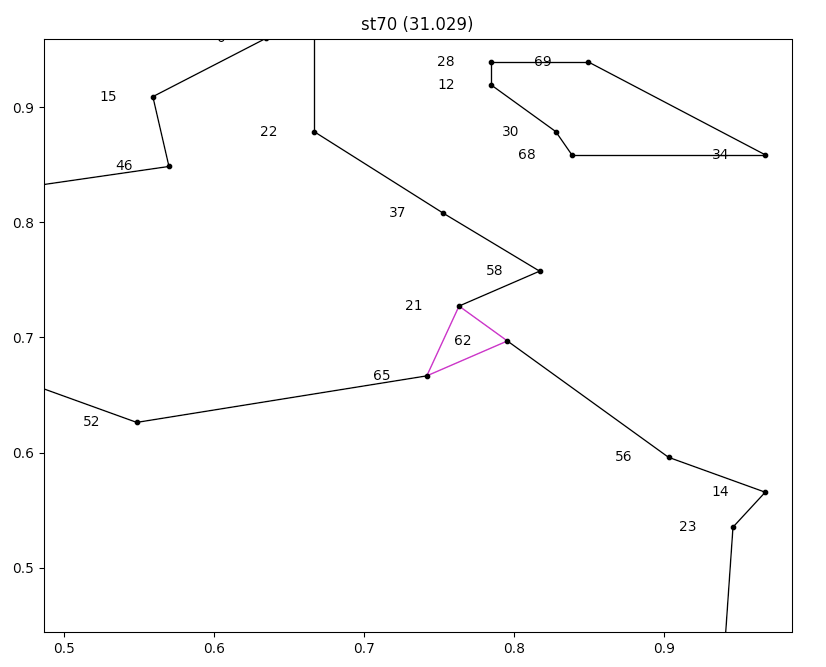
\includegraphics[width=1.5in, height=1.5in]{blossom_simple}
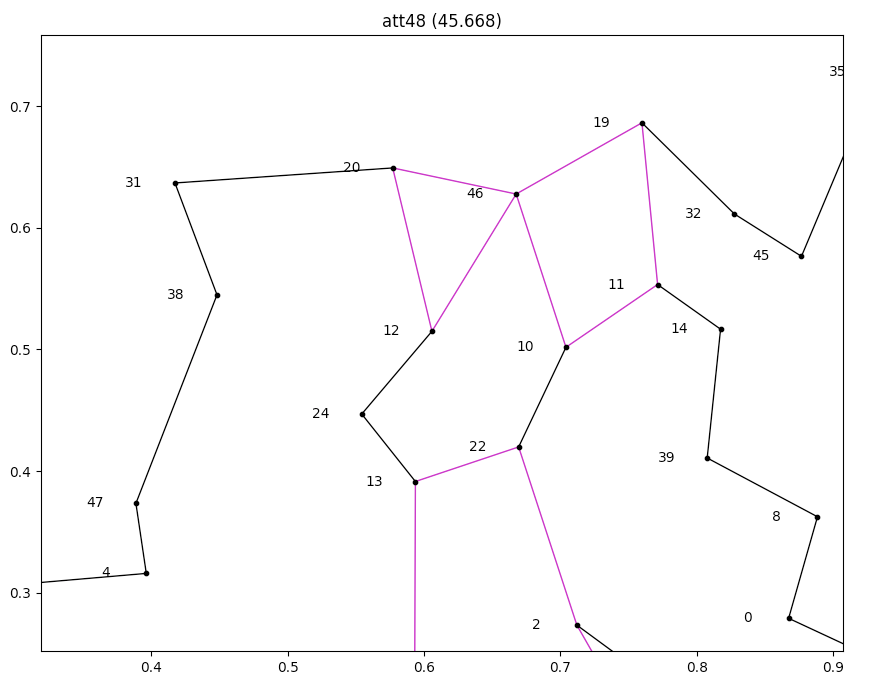
\includegraphics[width=1.5in, height=1.5in]{blossom_medium}
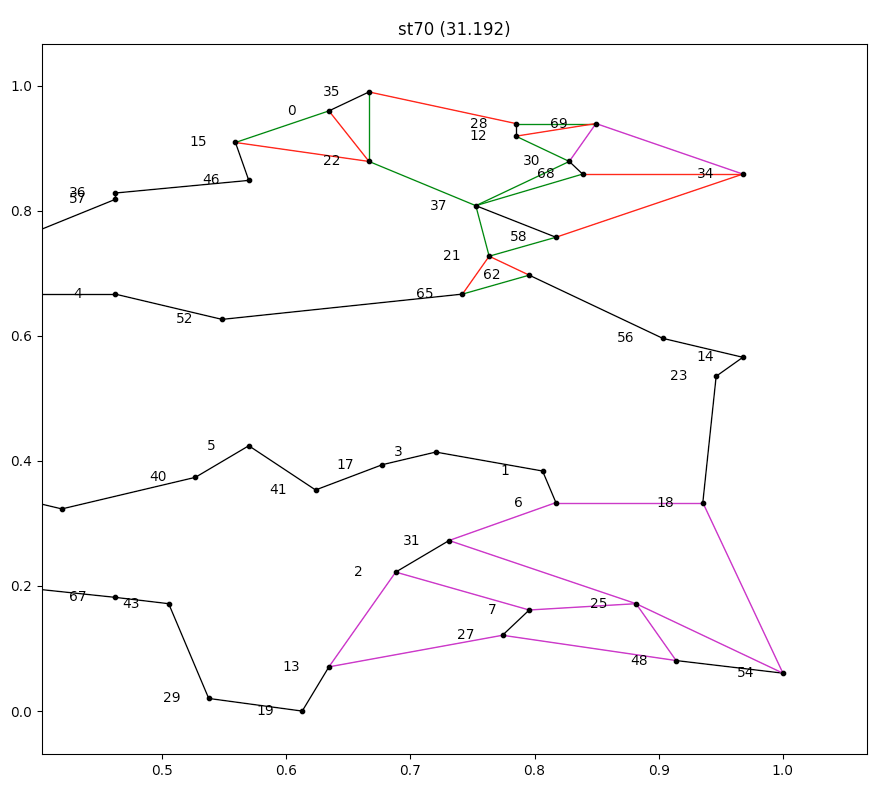
\includegraphics[width=1.5in, height=1.5in]{blossom_large}

\end{flushleft}

\subsection{Objective}

In our particular flavor of the TSP,
all edge costs $c_e$ are integral.
This implies that the objective value
of a valid TSP tour
must also be integral
because all $x_e$ decision variables
must be integral.

This makes it possible
to create a new constraint
whenever the LP relaxation objective value
is non-integral by just rounding it up:
\begin{equation}
\sum_{e \in E}{c_e x_e} >= \left \lceil \sum_{e \in E}{c_e x_e^*} \right \rceil
\end{equation}
where $x_e^*$ are the current LP relaxation decision variables.

It turns out that gurobi
allows constraints to be modified,
so only one objective constraint
is ever present at any given time.
Also, because this constraint relies
on locally-made decisions
(like variable fixing),
it is applied to the current model only.
Some precautions were taken
to avoid applying this constraint inappropriately
due to floating-point rounding issues.

\begin{lstlisting}
## tsp_solver.py
class TspBranchAndCut(object):
    def add_objective_constraints(self, model):
        obj_val = model.getAttr('ObjVal')
        ceil_obj_val  = math.ceil(obj_val)
        floor_obj_val = math.floor(obj_val)

        if (abs(obj_val - floor_obj_val) < 1e-6) or (abs(obj_val - ceil_obj_val) < 1e-6):
            return False

        target_constr_name = 'objective-roundup'

        target_constr = None
        for constr in model.getConstrs():
            if constr.getAttr('ConstrName') == target_constr_name:
                target_constr = constr
                break

        if target_constr is not None:
            target_constr.setAttr('RHS', ceil_obj_val)
        else:
            mvars = model.getVars()

            var_idxs = sorted([self.idx_by_edge[edge] for edge in self.edges])
            cvars = [mvars[idx].getAttr('Obj')*mvars[idx] for idx in var_idxs]

            model.addConstr(grb.quicksum(cvars) >= ceil_obj_val, 'objective-roundup')

        return True
\end{lstlisting}

\begin{flushleft}

\end{flushleft}

% \subsection{Gomory}
% \begin{flushleft}

% \end{flushleft}

\end{flushleft}

\section{Results}
\begin{flushleft}

The algorithms outlined above
were able to solve all assigned TSP datasets.

\begin{center}
\begin{tabular}{ l r r }
  dataset & time (sec) & optimal tour cost \\
  \hline
  att48 &     0.84 &  10628 \\
  berlin22 &  0.06 &   7542 \\
  gr21 &      0.01 &   2707 \\
  hk48 &      0.49 &  11461 \\
  pr76 &   4263.32 & 108159 \\
  st70 &      4.24 &    675 \\
  ulysses22 & 0.04 &   7013
\end{tabular}
\end{center}

Images and details of each tour
can be found in section \ref{sec:resultdetails}.

\end{flushleft}

\section{Future Improvements}

Clearly there is room for improvement on dataset pr76.

We performed an analysis to determine whether or not
using the Held-Karp algorithm could drive models
toward the optimum value more quickly,
but the Held-Karp bounds on these datasets
were not particularly close to the optima.

We also implemented Gomory mixed-integer cuts,
which were very successful on all datasets
except pr76, which we suspect might be due
to the accumulation of rounding errors.
The Gomory cuts could solve all other datasets
even with all other constraints removed
(except, of course, integral subtour detection)
quite quickly (on the order of a few seconds at most).
The code for these cuts is included,
though it was disabled for these runs.
Using purely integer-based cuts might work better
for this type of problem.

\section{Result Details} \label{sec:resultdetails}
\begin{flushleft}

\subsection{att48}
\begin{flushleft}

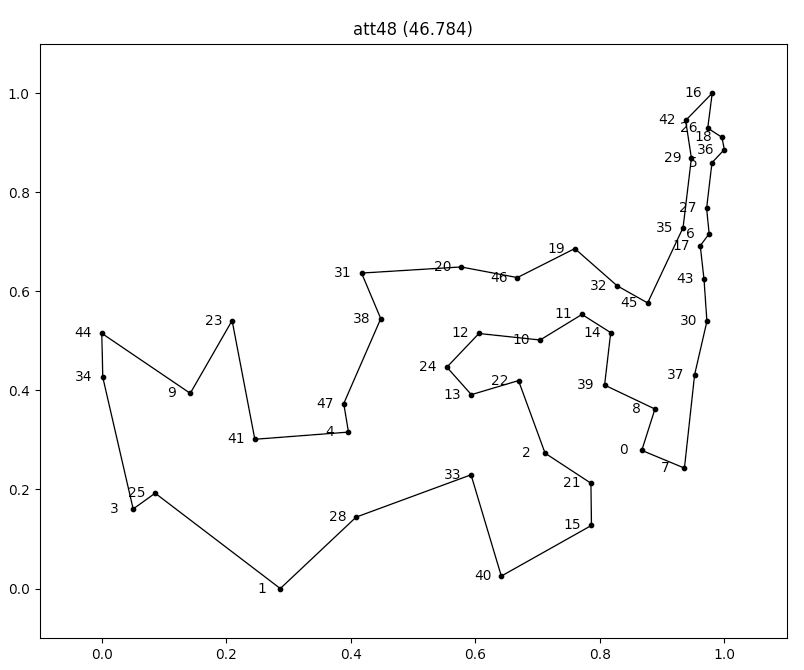
\includegraphics[width=4in, height=4in]{att48_optTour}

\begin{lstlisting}[language=C]
0   7   178
7   37  312
37  30  183
30  43  139
43  17  112
17  6   54
6   27  85
27  5   153
5   36  66
36  18  42
18  26  64
26  16  117
16  42  139
42  29  127
29  35  233
35  45  286
45  32  134
32  19  207
19  46  246
46  20  225
20  31  393
31  38  169
38  47  317
47  4   97
4   41  370
41  23  403
23  9   292
9   44  401
44  34  146
34  3   451
3   25  102
25  1   585
1   28  381
28  33  474
33  40  356
40  15  393
15  21  140
21  2   207
2   22  262
22  13  192
13  24  133
24  12  169
12  10  242
10  11  186
11  14  129
14  39  175
39  8   214
8   0   147
The cost of the best tour is: 10628.0
\end{lstlisting}

\end{flushleft}

\subsection{berlin52}
\begin{flushleft}

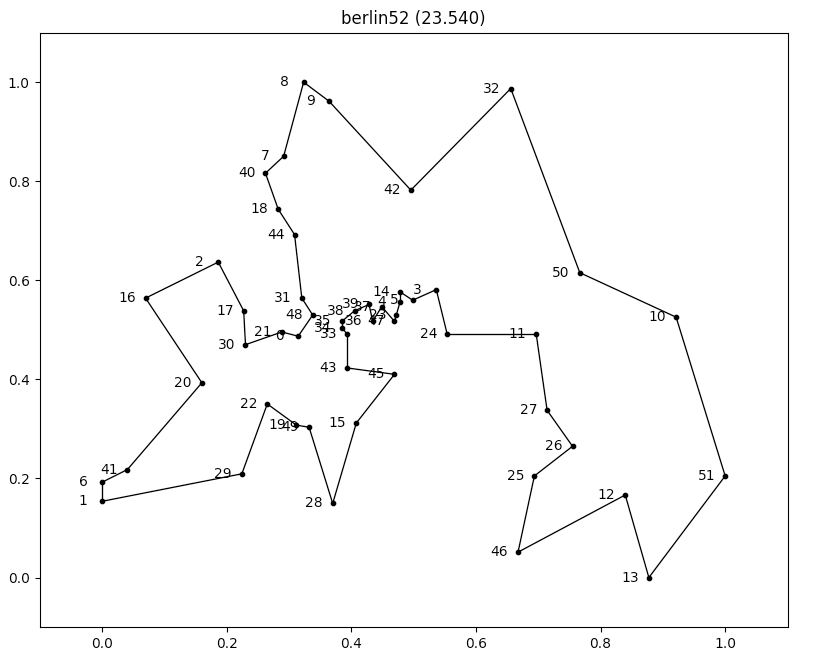
\includegraphics[width=4in, height=4in]{berlin52_optTour}

\begin{lstlisting}[language=C]
0   21  46
21  30  104
30  17  80
17  2   135
2   16  217
16  20  253
20  41  290
41  6   76
6   1   45
1   29  390
29  22  179
22  19  94
19  49  35
49  28  191
28  15  201
15  45  156
45  43  131
43  33  80
33  34  21
34  35  15
35  38  43
38  39  43
39  36  41
36  37  43
37  47  49
47  23  16
23  4   32
4   14  25
14  5   40
5   3   70
3   24  109
24  11  245
11  27  182
27  26  110
26  25  126
25  46  186
46  12  324
12  13  206
13  51  319
51  10  399
10  50  285
50  32  475
32  42  365
42  9   308
9   8   83
8   7   183
7   40  64
40  18  92
18  44  75
44  31  151
31  48  50
48  0   64
The cost of the best tour is: 7542.0
\end{lstlisting}

\end{flushleft}

\subsection{gr21}
\begin{flushleft}

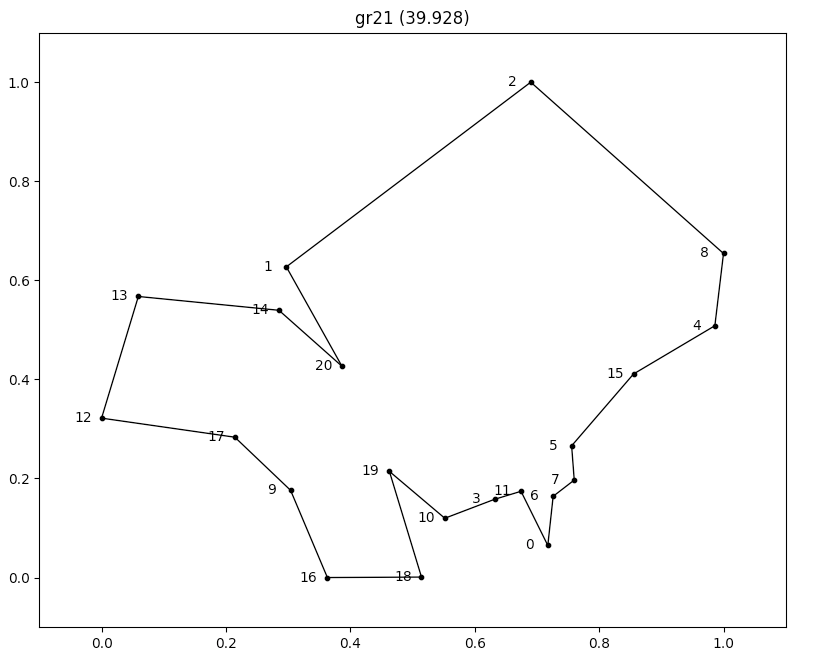
\includegraphics[width=4in, height=4in]{gr21_optTour}

\begin{lstlisting}[language=C]
0   6   110
6   7   29
7   5   36
5   15  125
15  4   125
4   8   120
8   2   295
2   1   355
1   20  140
20  14  105
14  13  170
13  12  190
12  17  180
17  9   77
9   16  150
16  18  87
18  19  155
19  10  100
10  3   63
3   11  27
11  0   68
The cost of the best tour is: 2707.0
\end{lstlisting}

\end{flushleft}

\subsection{hk48}
\begin{flushleft}

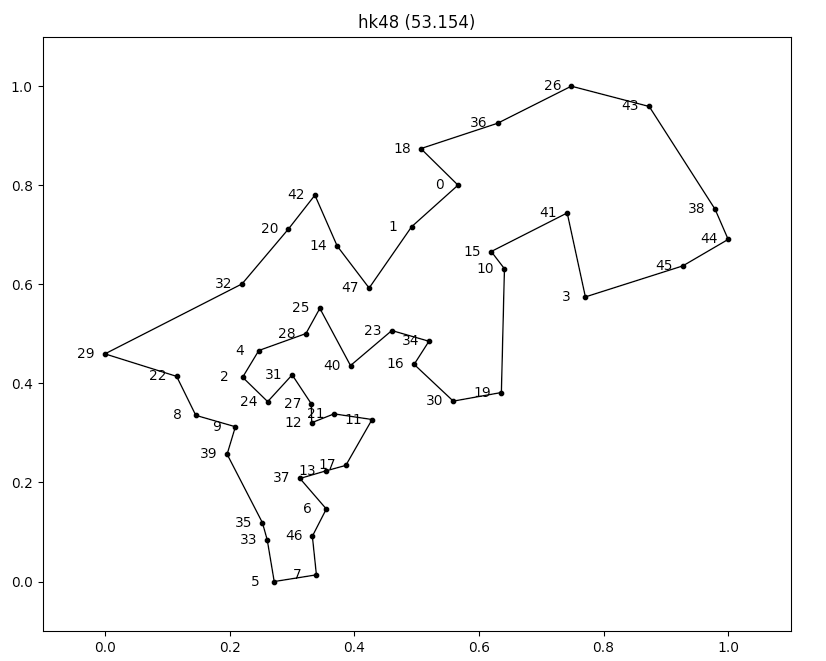
\includegraphics[width=4in, height=4in]{hk48_optTour}

\begin{lstlisting}[language=C]
0   1   273
1   47  335
47  14  236
14  42  252
42  20  189
20  32  318
32  29  669
29  22  326
22  8   197
8   9   177
9   39  130
39  35  345
35  33  83
33  5   188
5   7   182
7   46  177
46  6   138
6   37  178
37  13  115
13  17  90
17  11  238
11  21  165
21  12  100
12  27  90
27  31  154
31  24  161
24  2   155
2   4   140
4   28  217
28  25  129
25  40  291
40  23  238
23  34  166
34  16  123
16  30  235
30  19  214
19  10  563
10  15  96
15  41  371
41  3   387
3   45  443
45  44  229
44  38  145
38  43  534
43  26  347
26  36  357
36  18  346
18  0   229
The cost of the best tour is: 11461.0
\end{lstlisting}

\end{flushleft}

\subsection{pr76}
\begin{flushleft}

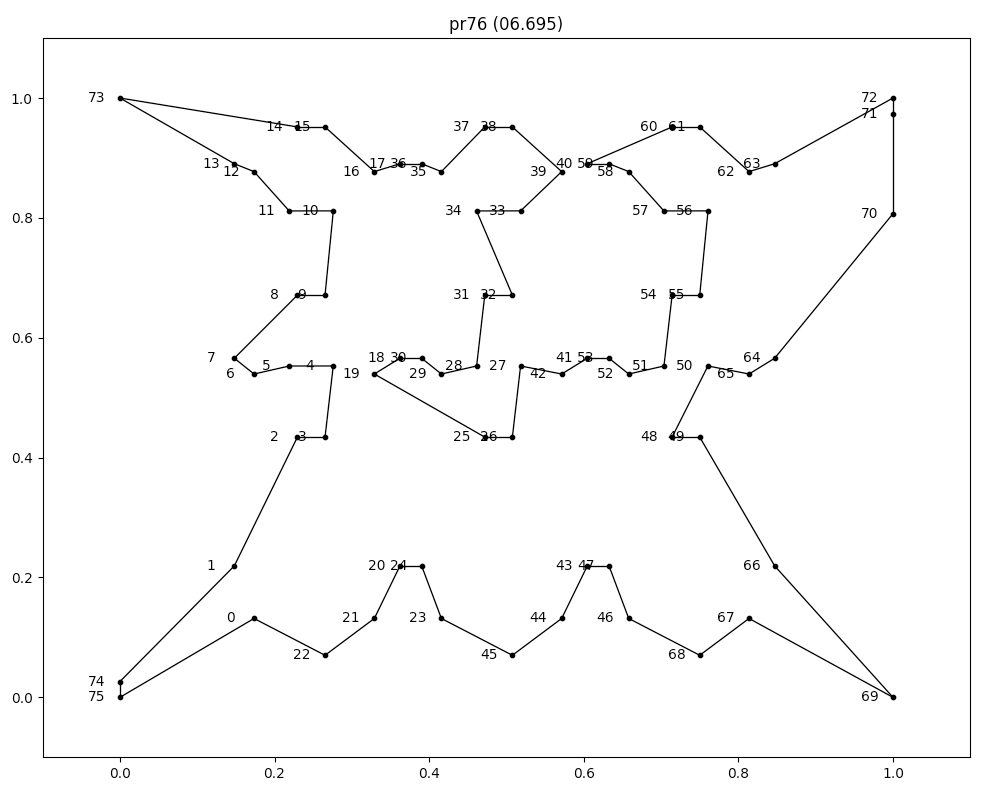
\includegraphics[width=4in, height=4in]{pr76_optTour}

\begin{lstlisting}[language=C]
0   22  1931
22  21  1433
21  20  1193
20  24  550
24  23  1118
23  45  1931
45  44  1433
44  43  1193
43  47  550
47  46  1118
46  68  1931
68  67  1433
67  69  3946
69  66  3905
66  49  3100
49  48  700
48  50  1629
50  65  1053
65  64  716
64  70  4070
70  71  1900
71  72  300
72  63  3250
63  62  667
62  61  1512
61  60  700
60  40  2261
40  59  550
59  58  522
58  57  1164
57  56  1118
56  55  1617
55  54  700
54  51  1364
51  52  906
52  53  583
53  41  550
41  42  716
42  27  1053
27  26  1369
26  25  700
25  19  3046
19  18  716
18  30  550
30  29  583
29  28  906
28  31  1364
31  32  700
32  34  1841
34  33  1118
33  39  1280
39  38  1512
38  37  700
37  35  1390
35  36  522
36  17  550
17  16  667
16  15  1512
15  14  700
14  73  4533
73  13  3158
13  12  522
12  11  1164
11  10  1118
10  9   1617
9   8   700
8   7   2000
7   6   583
6   5   906
5   4   1115
4   3   1369
3   2   700
2   1   2926
1   74  3640
74  75  300
75  0   3716
The cost of the best tour is: 108159.0
\end{lstlisting}

\end{flushleft}

\subsection{st70}
\begin{flushleft}

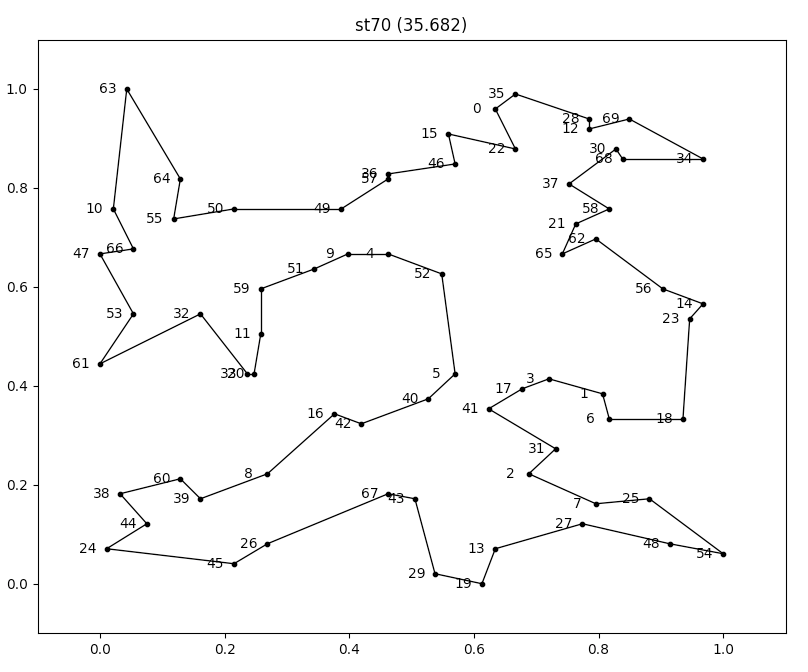
\includegraphics[width=4in, height=4in]{st70_optTour}

\begin{lstlisting}[language=C]
0   22  9
22  15  10
15  46  6
46  36  10
36  57  1
57  49  9
49  50  16
50  55  9
55  64  8
64  63  20
63  10  24
10  47  9
47  66  5
66  53  13
53  61  11
61  32  18
32  33  14
33  20  1
20  11  8
11  59  9
59  51  9
51  9   6
9   4   6
4   52  9
52  5   20
5   40  6
40  42  11
42  16  4
16  8   16
8   39  11
39  60  5
60  38  9
38  44  7
44  24  8
24  45  19
45  26  6
26  67  21
67  43  4
43  29  15
29  19  7
19  13  7
13  27  14
27  48  14
48  54  8
54  25  16
25  7   8
7   2   12
2   31  6
31  41  13
41  17  6
17  3   4
3   1   9
1   6   5
6   18  11
18  23  20
23  14  4
14  56  7
56  62  14
62  65  6
65  21  6
21  58  6
58  37  8
37  30  10
30  68  2
68  34  12
34  69  14
69  12  6
12  28  2
28  35  12
35  0   4
The cost of the best tour is: 675.0
\end{lstlisting}

\end{flushleft}

\subsection{ulysses22}
\begin{flushleft}

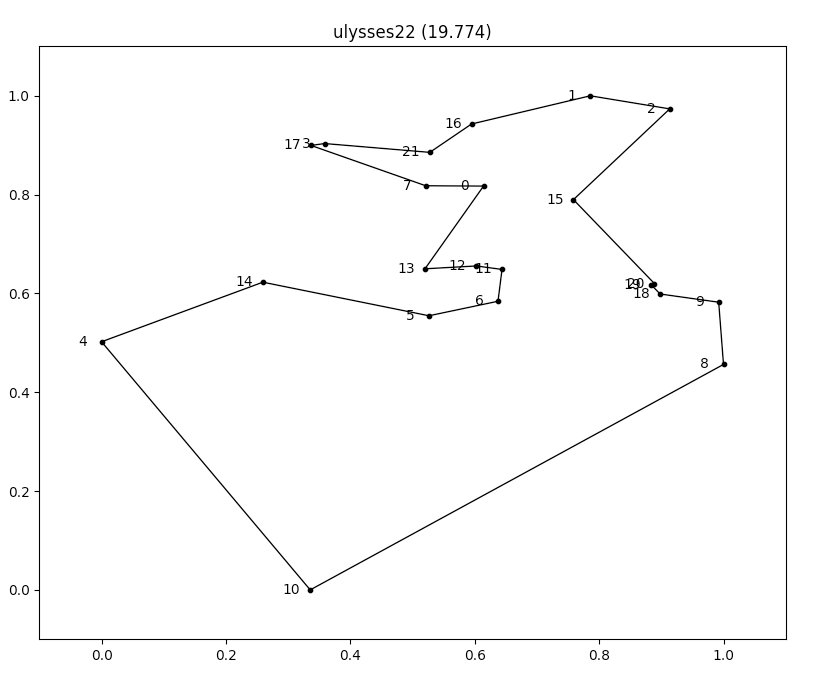
\includegraphics[width=4in, height=4in]{ulysses_optTour}

\begin{lstlisting}[language=C]
0   7   60
7   17  278
17  3   37
3   21  171
21  16  148
16  1   246
1   2   126
2   15  499
15  20  486
20  19  14
19  18  33
18  9   96
9   8   328
8   10  1387
10  4   1504
4   14  401
14  5   308
5   6   115
6   11  177
11  12  68
12  13  52
13  0   479
The cost of the best tour is: 7013.0
\end{lstlisting}

\end{flushleft}


\end{flushleft}




Once we developed our algorithm for solving TSPBC,
we looked to Python and the gurobipy module.
Additionally, we implemented a Graph object
to facilitate our computation of TSPBC.
Graph is initialized
by helper functions
that assign its node, edge and edge weight attributes.
Graph also contains
methods to find the minimum cut,
to compute connected components,
and to determine if the instance forms a tour.
Instances of graph are copied
before more branches are produced.
Additionally, there are auxiliary functions
that easily convert
a Graph instance into a Gurobi model.


\section{Constraints}
These specific cuts
are comb and blossom inequalities,
integral and non-integral sub-tour constraints,
and mixed-integer Gomory cuts.
For the comb and blossom inequalities,
we searched for cuts based of this equation
in our candidate solution:
[INSERT BLOSSOM INEQUALITY]
For both integral and non-integral sub-tour constraints,
we check to see
if the current model formed a sub-tour,
and if so we added a constraint.
Lastly, for mixed integer Gomory cuts,
we searched for cuts based of
[INSERT MIXED INTEGER GOMORY CUTS].
For each cut,
constraints are added
to each Gurobi model
and the model is then solved
and branched out again.

\section{Min Cut}
To compute the min cut,
we use the Stoer-Wagner min-cut algorithm
in the provided paper.
Our implementation of this algorithm
returned the nodes that made up the min cut
as well as the size of the min cut.
The value of the minimum cut
was less than two
if and only if
there is a constraint that has been violated.
This function is contained as a method in Graph.

\section{Computing Tour}
Given a candidate branch,
we must check if it forms a potential solution.
In our python implementation,
our solution is a vector of values in [0.0, 1.0].
These values represent
if an edge is included in our solution.
We can eliminate infeasible branches
if their vector contains a value
that isn’t either 0.0 or 1.0.
Additionally, we need to check
if our potential solution satisfies
the degree constraint [degree].
Finally, we must check
that our candidate solution produces
at most one connected component.
We can compute the connected components
of our candidate solution
by running breadth-first search
on every edge in our candidate solution.
If our candidate solution passes
that each edge is either 0.0 or 1.0,
then we have each node in our tour
meeting the degree constraint [degree],
and that our candidate solution
forms at most one connected components [degree],
then this is sufficient to declare
our candidate solution a tour.
This function is contained as a method in Graph.

\section{Implementation}

\subsection{The Graph Class}

A \textit{Graph} class was created
to encapsulate purely graph-related functionality,
such as identifying:
\begin{enumerate}
\item nodes in connected components
\item edges in a min-cut
\item edges in the cut for a set of nodes
\item whether or not a set of edges forms a tour
\end{enumerate}

\section{Results}
    att48

    berlin52

    gr21

    hk48

    ulysses22

    pr76

    st70

\section{Improvements}

\section{Closing Remarks}
Our implementation of TSPBC was successful
in that we could correctly solve
each of the data sets provided.
However, as stated in our improvements section,
we could have added more types of cuts
to reduce the runtime of pr76.


\section{Section Title Here}

\subsection{Subsection Title Here}

\begin{flushleft}

Some text here.

\begin{equation} \label{probdef}
  p(a \le Z \le b) = \int_{a}^{\,b} \phi(x) \,dx
\end{equation}

Reference equation \autoref{probdef} here.

\begin{align*}
  p(a \le Z \le b)  &=  p(Z \le b) - p(Z \le a) \\
                    &=  \int_{-\infty}^{\,b} \phi(x) \,dx
                        -
                        \int_{-\infty}^{\,a} \phi(x) \,dx \\
                    &=  \Phi(b) - \Phi(a)
\end{align*}

Inline $\Phi(\alpha)$ here.

\begin{equation*}
  \Phi(\alpha)  = \int_{-\infty}^{\,\alpha} \phi(x) \,dx
\end{equation*}

% \begin{figure}[h!]
% \begin{center}
% \input{fig_pdfcdfarea}
% \caption{
% Image caption here.}
% \label{pdfcdfarea}
% \end{center}
% \end{figure}

\end{flushleft}

\end{document}
